\documentclass[12pt]{article} % размер шрифта
% \usepackage{tikz} % картинки в tikz
\usepackage{graphicx}
\graphicspath{{images/}}
\usepackage{microtype} % свешивание пунктуации
\usepackage{array} % для столбцов фиксированной ширины
\usepackage{url} % для вставки ссылок \url{...}
\usepackage{indentfirst} % отступ в первом параграфе
\usepackage{sectsty} % для центрирования названий частей
\allsectionsfont{\centering} % приказываем центрировать все sections
\usepackage{amsthm} % теоремы и доказательства
\theoremstyle{definition} % прямой шрифт в условии теорем
\newtheorem{theorem}{Теорема}[section]
\usepackage{amsmath} % куча стандартных математических плюшек
\usepackage[top=2cm, left=1.5cm, right=1.5cm, bottom=2cm]{geometry} % размер текста на странице
\usepackage{lastpage} % чтобы узнать номер последней страницы
\usepackage{enumitem} % дополнительные плюшки для списков
%  например \begin{enumerate}[resume] позволяет продолжить нумерацию в новом списке
\usepackage{caption} % подписи к картинкам без плавающего окружения figure


\usepackage{fancyhdr} % весёлые колонтитулы
\pagestyle{fancy}
\lhead{Эконометрика, финтех}
\chead{}
\rhead{2018-09-22, встреча 1}
\lfoot{}
\cfoot{}
\rfoot{\thepage/\pageref{LastPage}}
\renewcommand{\headrulewidth}{0.4pt}
\renewcommand{\footrulewidth}{0.4pt}



\usepackage{todonotes} % для вставки в документ заметок о том, что осталось сделать
% \todo{Здесь надо коэффициенты исправить}
% \missingfigure{Здесь будет картина Последний день Помпеи}
% команда \listoftodos — печатает все поставленные \todo'шки

\usepackage{booktabs} % красивые таблицы
% заповеди из документации:
% 1. Не используйте вертикальные линии
% 2. Не используйте двойные линии
% 3. Единицы измерения помещайте в шапку таблицы
% 4. Не сокращайте .1 вместо 0.1
% 5. Повторяющееся значение повторяйте, а не говорите "то же"

\usepackage{fontspec} % поддержка разных шрифтов
\usepackage{polyglossia} % поддержка разных языков

\setmainlanguage{russian}
\setotherlanguages{english}

\setmainfont{Linux Libertine O} % выбираем шрифт
% если Linux Libertine не установлен, то
% можно также попробовать Helvetica, Arial, Cambria и т.Д.

% чтобы использовать шрифт Linux Libertine на личном компе,
% его надо предварительно скачать по ссылке
% http://www.linuxlibertine.org/index.php?id=91&L=1

% на сервисах типа sharelatex.com этот шрифт есть :)

\newfontfamily{\cyrillicfonttt}{Linux Libertine O}
% пояснение зачем нужно шаманство с \newfontfamily
% http://tex.stackexchange.com/questions/91507/

\AddEnumerateCounter{\asbuk}{\russian@alph}{щ} % для списков с русскими буквами
\setlist[enumerate, 2]{label=\asbuk*),ref=\asbuk*} % списки уровня 2 будут буквами а) б) ...

%% эконометрические и вероятностные сокращения
\DeclareMathOperator{\Cov}{Cov}
\DeclareMathOperator{\Corr}{Corr}
\DeclareMathOperator{\Var}{Var}
\DeclareMathOperator{\E}{E}
\def \hb{\hat{\beta}}
\def \hs{\hat{\sigma}}
\def \htheta{\hat{\theta}}
\def \s{\sigma}
\def \hy{\hat{y}}
\def \hY{\hat{Y}}
\def \v1{\vec{1}}
\def \e{\varepsilon}
\def \he{\hat{\e}}
\def \hu{\hat{u}}
\def \z{z}
\def \hVar{\widehat{\Var}}
\def \hCorr{\widehat{\Corr}}
\def \hCov{\widehat{\Cov}}
\def \cN{\mathcal{N}}


\begin{document}
Конспектировал: Всеволод Овечкин
\section{МНК без теории вероятности}

Регрессионный анализ используют в основном для:
\begin{enumerate}
    \item описания зависимости между признаками
    \item предсказания значений переменной
\end{enumerate}

В этом семинаре речь пойдет о методе наименьших квадратов (МНК) без теории вероятности, решении задачи поиска коэффициентов различными способами и геометрической интерпретации МНК.

\subsection{Пример выявления зависимости}

Рассмотрим небольшой пример, в котором $y$ - это количество составленных задач по эконометрике, $x$ - это количество съеденных пирожков. Попробуем выяснить как зависят эти две величины.

\begin{table}[h!]
    \centering
    \begin{tabular}{c|c}
        \hline
        y & x \\
        \hline
        10 & 5 \\
        14 & 6 \\
        5 & 2
    \end{tabular}
    \caption{Зависимость количества составленных задач по эконометрике от количества съеденных пирожков.}
    \label{fist_table}
\end{table}

Введем обозначения $y_i$ - фактическое значение объясняемой переменной, $\hy_i$ - предсказанное значение объясняемой переменной, $\hu_i$ - ошибка предсказания.
\[
y = \begin{bmatrix}
           y_{1} \\
           y_{2} \\
           \vdots \\
           y_{n}
         \end{bmatrix}; 
\hy = \begin{bmatrix}
           \hy_{1} \\
           \hy_{2} \\
           \vdots \\
           \hy_{n}
         \end{bmatrix}; 
\hu_i = y_i - \hy_i; 
\hu = \begin{bmatrix}
           \hu_{1} \\
           \hu_{2} \\
           \vdots \\
           \hu_{n}
         \end{bmatrix}
\]

Предположим, что зависимость выглядит следующим образом

\[
\hy_i = \hb x_i
\]

Как найти $\hb$?. МНК метод позволяет найти такую $\hb$, чтобы сумма квадратов ошибок была минимальна. Математически эту идею можно выразить несколькими способами:

\[
\sum_{i=1}^n \left( y_i - \hy_i \right)^2 \rightarrow \underset{\hb}{min}
\]
\[
d^2(y,\hy) \rightarrow \underset{\hb}{min}
\]
\[
\left( y-\hy\right)^T\left( y-\hy\right) \rightarrow \underset{\hb}{min}
\]

Решим задачу минимизации суммы:

\[
Q(\hb) = \sum_{i=1}^n \left( y_i - \hy_i \right)^2 = 
\sum_{i=1}^n \left( y_i - \hb x_i \right)^2 = 
\sum_{i=1}^n \left( y_i - 2y_i\hb x_i + (\hb x_i)^2 \right)\rightarrow \underset{\hb}{min}
\]

\[
Q'(\hb) = \sum_{i=1}^n \left( - 2y_i x_i + 2\hb x_i \right) 
\]

Найдем условие первого порядка:

\[
\sum_{i=1}^n \left( - 2y_i x_i + 2\hb x_i \right) = 0
\]
\[
-2\sum_{i=1}^n y_i x_i + 2\hb \sum_{i=1}^n x_i  = 0
\]
\[
\hb   = \frac{\sum_{i=1}^n y_i x_i}{\sum_{i=1}^n x_i}
\]

\[
\hb   = \frac{50+84+10}{25+36+4} = 2.215
\]

Таким образом уравнение, позволяющее описать линейную зависимость $y$ от $x$, и минимизирующее сумму квадратов остатков, выглядит следующим образом:
\[
\hy = 2.215*x 
\]

\subsection{Матричное дифференцирование}

Пусть есть:
\[
F =  \begin{bmatrix}
        x_1 + x_2  & 2x_1^2 \\
        x_1x_2    & cos(x_2)\\
         \end{bmatrix}
\]

Тогда: 
\[
dF =  \begin{bmatrix}
        dx_1 + dx_2  & 4x_1dx_1 \\
        x_1dx_1+x_2dx_2    & -sin(x_2)dx_2\\
         \end{bmatrix}
\]

\begin{table}[h!]
    \centering
    \begin{tabular}{c|c}
        \hline
        Скаляр & Матрица  \\
        \hline
        $d(a+b) = da + db$ & $d(A+B) = dA + dB$\\
        $d(ab) = bda + adb$ & $d(AB) = dAB + AdB$\\
        $d(cb) = cdb, c=const$ & $d(CB) = CdB, C=const$ \\
        & $d(A^T)=(dA)^T$
    \end{tabular}
    \caption{Сравнение операций дифференцирования скаляра и матрицы}
    \label{third_table}
\end{table}

Задачу поиска $\hb$ так же можно решить при помощи матричного дифференциала:

\[
Q(\hb) = \left( y-\hy\right)^T\left( y-\hy\right) \rightarrow \underset{\hb}{min}
\]
\begin{eqnarray*}
dQ(\hb) = d( y-x\hb)^T( y-x\hb) + ( y-x\hb)^Td( y-x\hb) = \\
=(-xd\hb)^T( y-x\hb) + (y-x\hb)^T(-xd\hb)=\\
=-2(y-x\hb)^T(xd\hb)
\end{eqnarray*}

Найдем условие первого порядка. Так как для любого $d\hb$ должно выполняться $dQ(\bh)=0$, то

\[
-2(y-x\hb)^Tx = 0
\]
\[
x^T(y-x\hb) = 0
\]
\[
x^Ty-x^Tx\hb = 0
\]
\[
x^Tx\hb = x^Ty
\]
\[
\hb = \frac{x^Ty}{x^Tx}
\]

\subsection{Упражнения на матричное дифференцирование}

Найти $dA^{-1}$, зная 

\[
I_{n,n} =  \begin{bmatrix}
           1 & 0 & \hdots & 0 \\
           0 & 1 & \hdots & 0 \\
           \vdots & \vdots & \ddots & \vdots \\
            0 & 0 & \hdots & 1 \\
         \end{bmatrix};
dI = 0;
dA
\]

Решение:

\[
dI = d(AA^{-1}) = dAA^{-1} + AdA^{-1} = 0
\]
\[
dAA^{-1} = -AdA^{-1}
\]
\[
dA{-1} = -A^{-1}dA^{-1}
\]

\section{МНК с несколькими регрессорами}

Пусть имеются данные:

\begin{table}[h!]
    \centering
    \begin{tabular}{c|c|c}
        \hline
        y & x & z \\
        \hline
        \vdots & \vdots & \vdots
    \end{tabular}
    \caption{Случайные данные}
    \label{second_table}
\end{table}

Предположим, что мы хотим оценить уравнение регрессии:
\[
\hy_i = \hb_1 + \hb_2 x_i + \hb_3 z_i
\]

Введем обозначения: $k$ - количество коэффициентов, $n$ - количество наблюдений. Тогда

\[
y = \begin{bmatrix}
           y_{1} \\
           y_{2} \\
           \vdots \\
           y_{n}
         \end{bmatrix}; 
\hy = \begin{bmatrix}
           \hy_{1} \\
           \hy_{2} \\
           \vdots \\
           \hy_{n}
         \end{bmatrix};
X =  \begin{bmatrix}
           1 & x_1 & z_1 \\
           1 & x_2 & z_2 \\
           \vdots & \vdots & \vdots \\
           1 & x_n &  z_n \\
         \end{bmatrix};
\hb = \begin{bmatrix}
           \hb_{1} \\
           \hb_{2} \\
           \hb_{3}
         \end{bmatrix}
\]

Уравнение регрессии можно записать в виде:
\[
\hy = X\hb
\]

Найдем методом МНК вектор $\hb$:
\begin{eqnarray*}
dQ(\hb) = d( y-X\hb)^T( y-X\hb) + ( y-X\hb)^Td( y-X\hb) = \\
=(-Xd\hb)^T( y-X\hb) + (y-X\hb)^T(-Xd\hb)=\\
=-2(y-X\hb)^T(Xd\hb)
\end{eqnarray*}

Найдем условие первого порядка. Так как для любого $d\hb$ должно выполняться $dQ(\bh)=0$, то

\[
-2(y-X\hb)^TX = 0
\]
\[
X^T(y-X\hb) = 0
\]
\[
X^Ty-X^TX\hb = 0
\]
\[
X^TX\hb = X^Ty
\]

В случае если $X^TX$ - обратима и $det(X^TX) \neq 0$, то
\[
\hb = (X^TX)^{-1}X^Ty
\]

\section{Геометрическая интерпретация МНК}

\[
\hY = \hb_1 \overline{1} + \hb_2 x 
\]

где, $\overline{1}$ - вектор столбец из единиц длинны $n$.
Описанное выше можно переформулировать следующим образом $\hy \in Lin(\overline{1}, x)$. Или $\hy$ - проекция $y$ на $Lin(\overline{1}, x)$

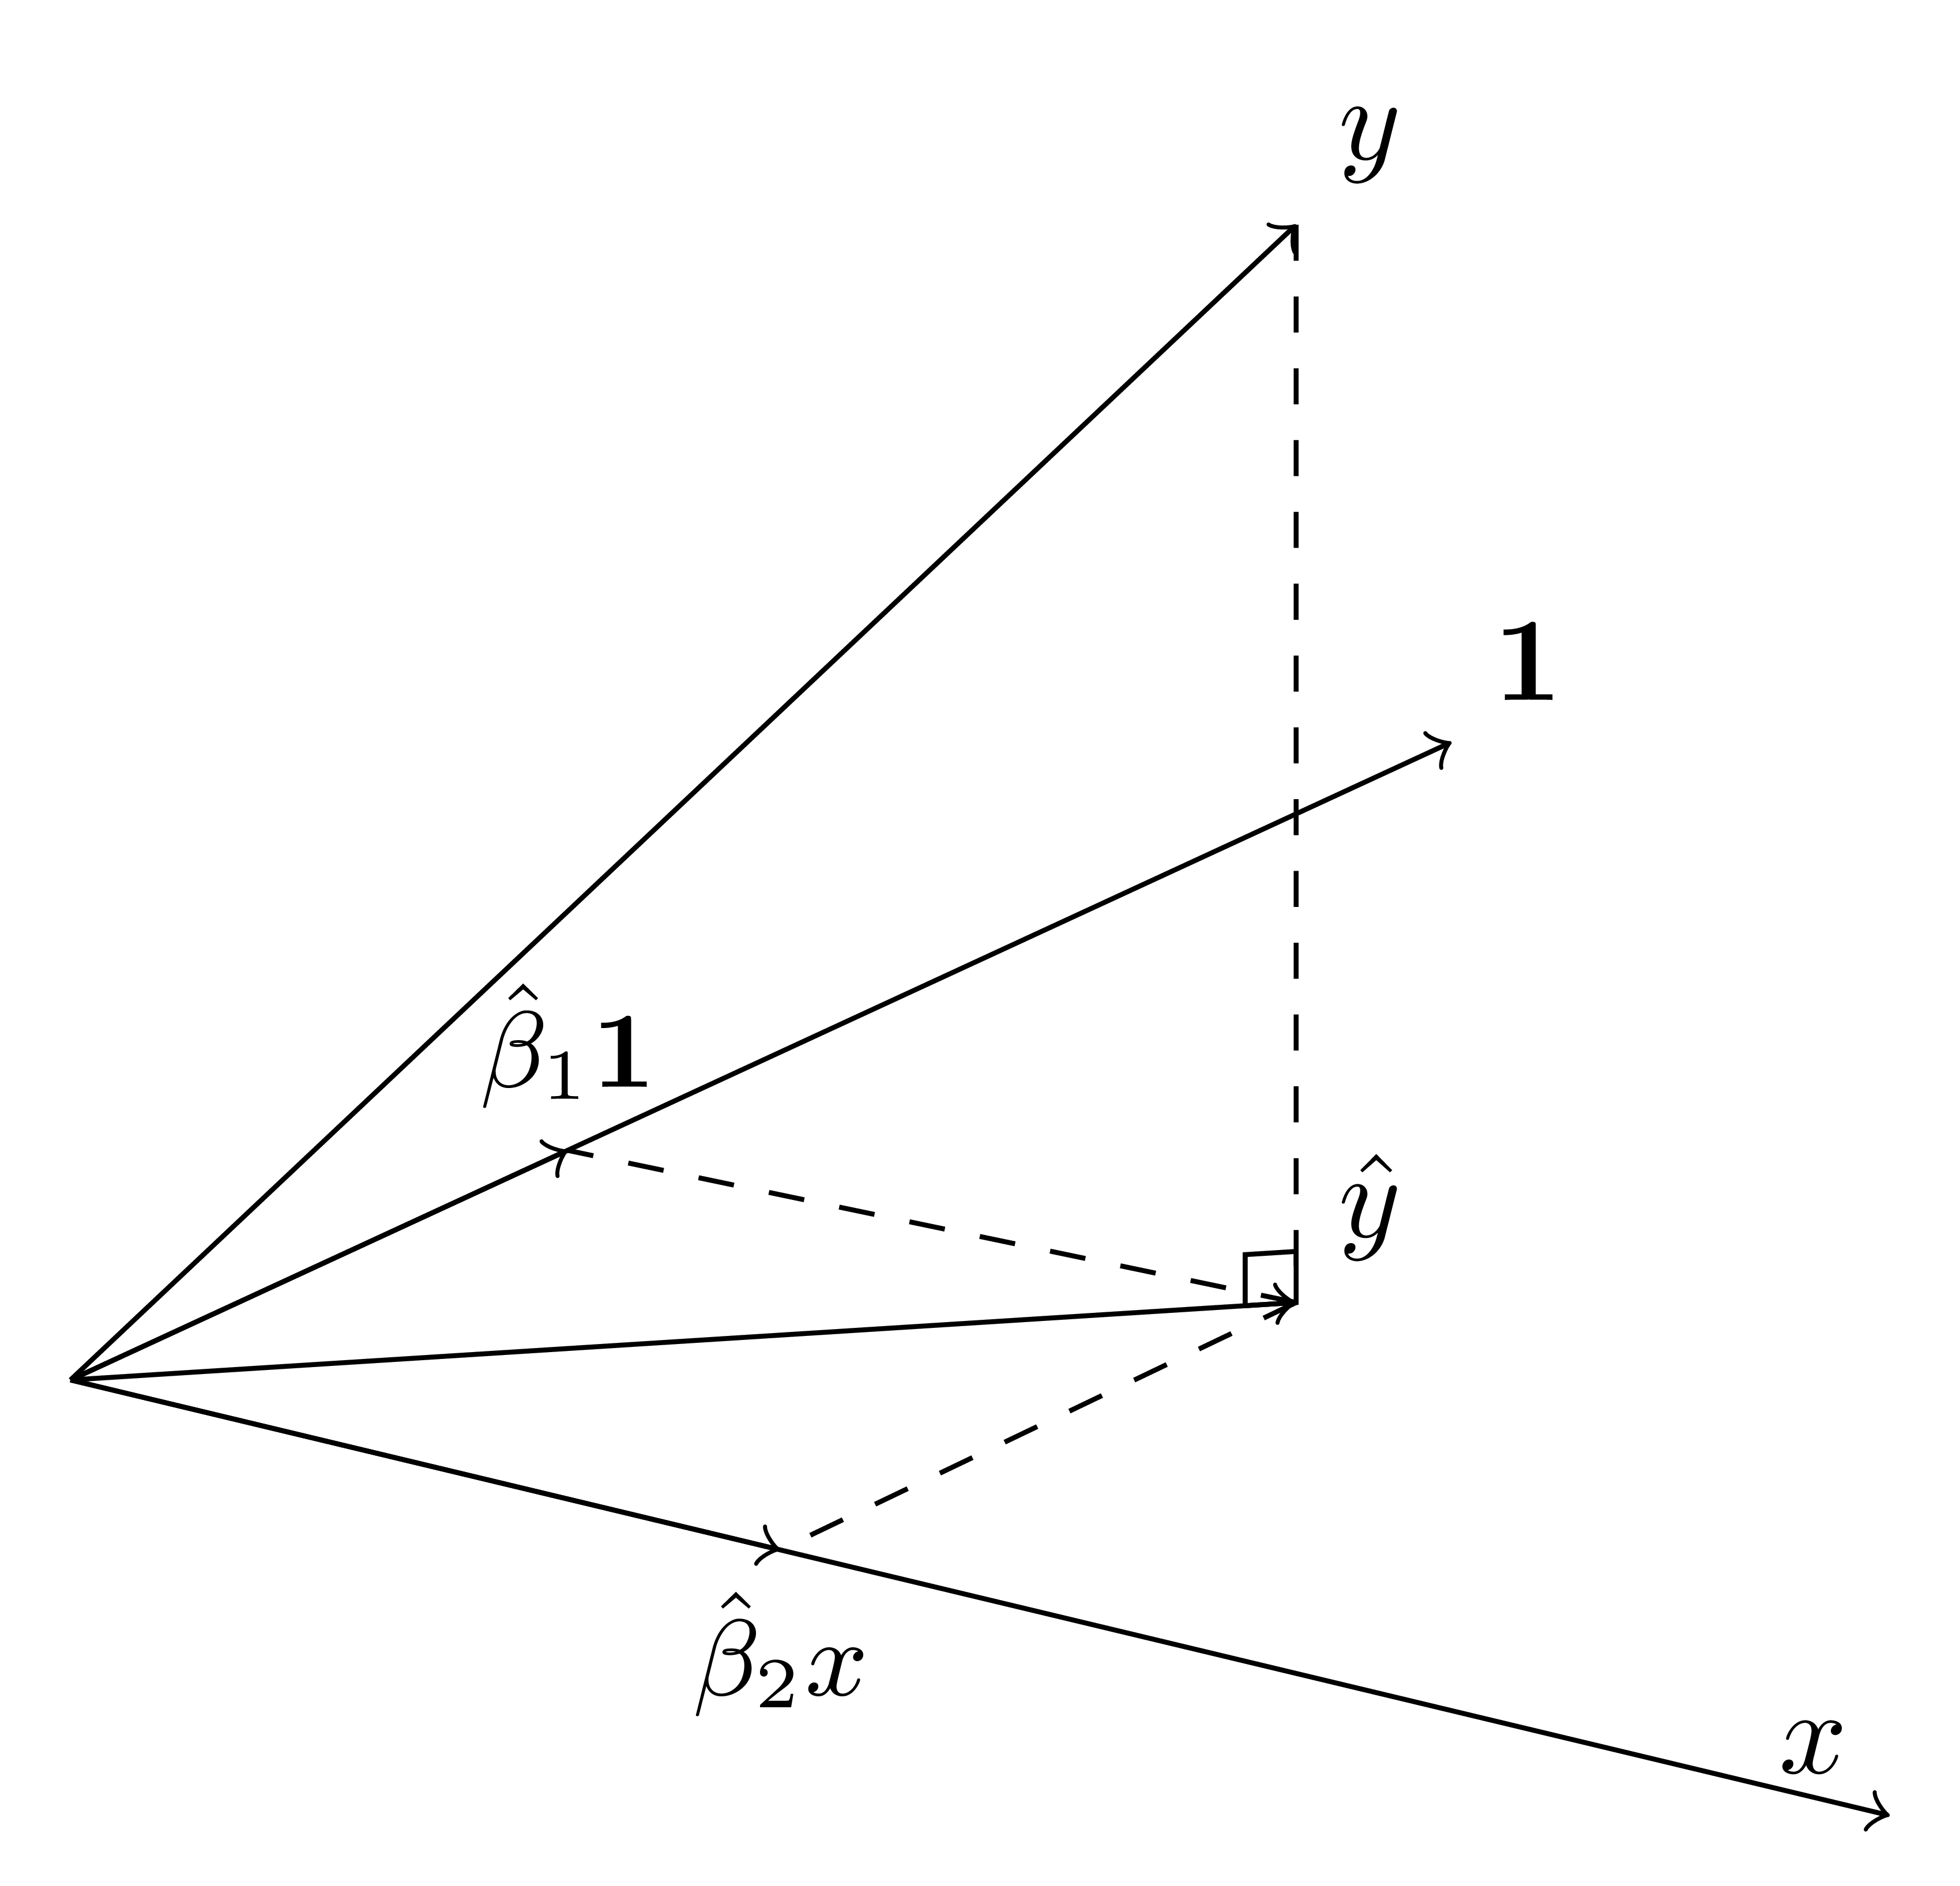
\includegraphics[width=10cm]{02_averages_yhat_decomposed}

Так же из рисунка видно, что вертор ошибок $\hu$ перпендикулярен $\hy$ и подпространству $Lin(\overline{1}, x)$ Поэтому геометрический смысл условий первого порядка можно выразить следующим образом:

\begin{equation*}
 \begin{cases}
   \overline{1}\hu = 0 \\
   x^T\hu = 0
 \end{cases}
 \Leftrightarrow
 X^T\hu = 0
\end{equation*}

\section{Коэффициент детерминации. Геометрическая интерпретация}


\includegraphics[width=10cm]{02_determination_coefficient}

Возьмем тривиальную модель:
\[
\hy = \hb_1 \overline{1}
\]

В этой простой модели решение будет выглядеть следующим образом:
\[
\hb = \frac{\overline{1}^Ty}{\overline{1}^T\overline{1}}
\]

Тогда $\hy$ можно будет найти по формуле:

\[
\hy = \overline{1} * \frac{\overline{1}^Ty}{\overline{1}^T\overline{1}} = \overline{1} *\frac{\sum y_i}{n} = \overline{1} *\overline{y}
\]

где, $\overline{y}$ - среднее значение $y$.

Вектор $\overline{1}\overline{y}$ на рисунке выше будет являть проекцией $\hy$ на вектор $\overline{1}$. А так как $\hy$ является проекцией $y$ на пространство $Lin(\overline{1}, x)$, то вектор $\overline{1} *\overline{y}$ тоже будет являться проекцией $y$ на вектор $\overline{1}$. Полученный треугольник с ребрами $a$, $b$, $c$ является прямоугольным.

Предположим, что мы оцениваем какую-то линейную (не тривиальную) модель. Предсказанные значений $y$ этой моделью обозначим как $\hy$. Тогда стороны треугольника можно интерпретировать следующим образом:

\begin{itemize}
    \item $||b||^2$ = $\sum_i (y_i - \overline{y})^2 = TSS$ (total sum of squares) - максимально возможная сумма квадратов ошибок модели при условии, что значения $\hy$ прогнозируются тривиальной моделью;
    \item $||a||^2$ = $\sum_i (y_i - \hy_i)^2 = RSS$ (residual sum of squares) - остаточная сумма квадратов, являющаяся суммой квадратов ошибок ($\hu$) модели;
    \item $||c||^2$ = $\sum_i (\hy_i - \overline{y})^2 = ESS$ (explained sum of squares) - объясненная сумма квадратов, показывающая часть TSS, которую удалось объяснить моделью;
\end{itemize}

По теореме Пифагора получаем: $TSS = ESS + RSS$. Тогда то, на сколько лучше наша модель предсказывает $y$ по сравнению с тривиальной моделью можно измерить коэффициентом детерминации:
\[
R^2 = \frac{ESS}{TSS} = 1- \frac{RSS}{TSS};
R^2 \in [0,1]
\]
Важное замечание: данная формула корректна в случае наличия $\overline{1}$ в модели.

\section{Упражнения на проекцию вектора на линейное подпространство}

Матрицей шляпницей будем называть матрицу, которая выполняет следующую функцию
\[
Hy=\hy
\]

В задаче регрессии эта матрица является выражается через X
\[
Hy=\hy=X\hb = X(X^YX)^{-1}X^Ty
\]
\[
H = X(X^YX)^{-1}X^T
\]

Чему равны следующие выражения:
\begin{enumerate}
    \item $H^2$ = ?
    \item $H^{2018}$ = ?
    \item $(I-H)^2$ = ?
\end{enumerate}

\textbf{Решение:} 
1-й пример это двойная проекция на $Lin(X)$, поэтому $H^2 = H$, так как проекция уже спроецированного вектора в $Lin(X)$ совпадает с этим вектором. 2-й пример решатся ровно так же $H^{2018}=H$. В 3-м примере матрица $(I-H)$ является проекцией на ортогональное дополнение $Lin(X)$, т.е. проекция является вектором ошибок. Поэтому $(I-H)^2$ является двойной проекцией на ортогональное дополнение $Lin(X)$, т.е. $(I-H)^2=(I-H)$

\section{Геометрическая интерпретация транспонирования}

Операцию транспонирования можно определить при помощи скалярного произведения не прибегая к фразе "переставление столбцов и строк местами".

Пусть есть 2 вектора $x$ и $y$. Предположим над вектором $x$ совершили преобразование $A$. Какое нужно совершить преобразование $B$ над вектором $y$ для того, чтобы выполнилось равенство:
\[
<Ax,y>=<x,By>
\]
Представим скалярное произведение в алгебраическом виде:
\[
(Ax)^Ty=x^TBy
\]
\[
x^TA^Ty=x^TBy
\]
Отсюда очевидно, что $B=A^T$.
\end{document}